\documentclass[a4paper,11pt]{article}
		\usepackage[utf8]{inputenc}
	\usepackage[italian]{babel}
	\usepackage{hyperref}	%Consente l'inserimento di \url
	\usepackage{booktabs}	%Utilità di abbellimento tabelle
	\usepackage{longtable}
	\usepackage{tabularx}
	%\usepackage{widetable}
	\usepackage{array}
	\usepackage{listings}
	\usepackage{graphicx}
	\usepackage{caption}
	\usepackage{fancyhdr}
	\newenvironment{fixpic}{}{} % [1]
	\usepackage[a4paper,top=3cm,bottom=3cm,left=2.5cm,right=2.5cm]{geometry}
	%******
	\usepackage{makeidx}
	\usepackage{textcomp}
	\usepackage{multirow}
	\usepackage{rotfloat}
	\usepackage{lastpage}
	\usepackage{array}
	\usepackage{float}
	% *************************************
	% QUI CODICE PER \SUBSUBSUBSECTION
	\usepackage{titlesec}
	\titleclass{\subsubsubsection}{straight}[\subsection]
	
	\newcounter{subsubsubsection}[subsubsection]
	\renewcommand\thesubsubsubsection{\thesubsubsection.\arabic{subsubsubsection}}
	\renewcommand\theparagraph{\thesubsubsubsection.\arabic{paragraph}} % optional; useful if paragraphs are to be numbered
	
	\titleformat{\subsubsubsection}
	  {\normalfont\normalsize\bfseries}{\thesubsubsubsection}{1em}{}
	\titlespacing*{\subsubsubsection}
	{0pt}{3.25ex plus 1ex minus .2ex}{1.5ex plus .2ex}
	
	\makeatletter
	\renewcommand\paragraph{\@startsection{paragraph}{5}{\z@}%
	  {3.25ex \@plus1ex \@minus.2ex}%
	  {-1em}%
	  {\normalfont\normalsize\bfseries}}
	\renewcommand\subparagraph{\@startsection{subparagraph}{6}{\parindent}%
	  {3.25ex \@plus1ex \@minus .2ex}%
	  {-1em}%
	  {\normalfont\normalsize\bfseries}}
	\def\toclevel@subsubsubsection{4}
	\def\toclevel@paragraph{5}
	\def\toclevel@paragraph{6}
	\def\l@subsubsubsection{\@dottedtocline{4}{7em}{4em}}
	\def\l@paragraph{\@dottedtocline{5}{10em}{5em}}
	\def\l@subparagraph{\@dottedtocline{6}{14em}{6em}}
	\makeatother
	
	\setcounter{secnumdepth}{4}
	\setcounter{tocdepth}{4}
	%FINE \SUBSUBSUBSECTION
	%****************************************
	%STYLE PER INSERIMENTO DEL CODICE
	\lstdefinestyle{style1}{
	  belowcaptionskip=1\baselineskip,
	  breaklines=true,
	  frame=L,
	  xleftmargin=\parindent,
	  language=Pascal,
	  showstringspaces=false,
	  basicstyle=\footnotesize\ttfamily,
	  keywordstyle=\bfseries\color{blue},
	  commentstyle=\itshape\color{blue},
	  identifierstyle=\color{blue},
	  stringstyle=\color{orange},
	}
	
	\lstdefinestyle{style2}{
	  belowcaptionskip=1\baselineskip,
	  frame=L,
	  xleftmargin=\parindent,
	  language=C,
	  basicstyle=\footnotesize\ttfamily,
	  commentstyle=\itshape\color{blue},
	}
	\lstset{style=style1}
	
	%FINE STYLE INSERIMENTO CODICE
	%*****************************************
	\usepackage[default]{cantarell} %% Use option "defaultsans" to use cantarell as sans serif only
	\usepackage[T1]{fontenc}        %% for font
	\hypersetup{colorlinks, linkcolor=black, urlcolor=blue}
	\newcommand{\addglos}{\begin{scriptsize}{\textbf{\ped{G}}} \end{scriptsize}} 
	\pagestyle{fancy}
	\fancyhead{}
	\fancyfoot{}
	%\fancyhead[L]{
\includegraphics[scale=0.28]{team_not_found.jpeg}}
	\fancyhead[L]{
\includegraphics[scale=0.15]{../../team404_small.jpg} \hspace{2mm} QUIZZIPEDIA}
	\fancyhead[R]{\leftmark}
	\fancyfoot[L]{Universit\`a degli studi di Padova - IS 2015/2016 \\ \url{team404swe@gmail.com}}

	
	%Commando usato per la tabella di informazioni sul documento
	\newcommand{\introtab}[9]{
		\begin{table}[ht]
		\begin{center}		
		\begin{tabular}{r l}			
			\toprule		
			\multicolumn{2}{c}{\textbf{ Informazioni sul documento }} \\
			\midrule 
			\textbf{Nome Documento}			& \vline \hspace{3.5 mm} {#1} \\
			\textbf{Versione}				& \vline \hspace{3.5 mm} {#2} \\
			\textbf{Uso} 					& \vline \hspace{3.5 mm} {#3} \\
			\textbf{Data Creazione} 		& \vline \hspace{3.5 mm} {#4} \\
			\textbf{Data Ultima Modifica} 	& \vline \hspace{3.5 mm} {#5} \\
			\textbf{Redazione}				& \vline \hspace{3.5 mm} {#6} \\
											%& \vline \hspace{3.5 mm} {#7} \\	
			\textbf{Verifica} 				& \vline \hspace{3.5 mm} {#7}	\\
			\textbf{Approvazione}			& \vline \hspace{3.5 mm} {#8}\\	
			\textbf{Committente} 			& \vline \hspace{3.5 mm} Zucchetti SPA\\
			\textbf{Lista di distribuzione} & \vline \hspace{3.5 mm} Prof. Vardanega Tullio \\														& \vline \hspace{3.5 mm} TEAM404 \\
	\bottomrule	
	\end{tabular}
	\end{center}
	\end{table}
	}
	% Comando di inizio del registro
	\newcommand{\beginregistro}{
		%\begin{longtable}{{|p{0.10\textwidth}|p{0.20\textwidth}|p{0.15\textwidth}|p{0.50\textwidth}|}}
		\begin{longtable}{{|p{1.5cm}|p{2.5cm}|p{2cm}|p{8cm}|}} 
	 		\hline	
	}
	% commando usato pr inserire una riga al registro delle modifiche
	\newcommand{\rigaregistro}[4]{
		{\footnotesize #1} & {\footnotesize #2} &  {\footnotesize #3} &  {\footnotesize #4} \\
			\hline	
	}
	% Comando di fine registro
	\newcommand{\fineregistro}{ \end{longtable}	}
	
	%************************************************
	% commandi per il GLOSSARIO
	%***********************************************
	% Commando di inizio tabella Glossario
	\newcommand{\beginglos}{
		\begin{longtable}{{p{0.20\textwidth}p{0.65\textwidth}}}	
	}
	% Commando per i termini del glossario
	
	\newcommand{\itemglos}[2]{
		\textbf{#1 :} & {#2} \\ \\ \\
	}
	% Commando fine Glossario
	\newcommand{\fineglos}{ \end{longtable} }
	% Comando per aggiungere una ssezione numerata con lettere al glossario
	\newcommand{\sezione}{
	\subsection{}	
	\rule[0.3pt]{\linewidth}{0.4pt} \\ % Linea orizzontale
	}
	
\newcommand{\sezioneglos}[1] { 
  \newpage
  \cleardoublepage
  \phantomsection
  \addcontentsline{toc}{section}{#1}
  \vspace{11pt}
  \textbf{\huge{#1} } % Lettera grande 
  \\
  \rule[0.3pt]{\linewidth}{0.4pt} \\ % Linea orizzontale
  \fancyhead[R]{#1}
}
	\newcommand{\code}[1]{\texttt{#1}}

	\title{\textbf{{\fontsize{8mm}{5mm}\selectfont QUIZZIPEDIA}}}
	\date{}
	\author{}	


\begin{document}
	\maketitle
	\thispagestyle{empty}
	\begin{center}	
	
\includegraphics{../team_not_found.jpg}\\
	\fontsize{5mm}{3mm}\url{team404swe@gmail.com}\\
	
	\vspace{50mm}
	\textbf{Definizione di Prodotto 1.0}
	\end{center}
	\introtab{Definizione di Prodotto}	%1 nome documento
			{1.0} 							%2 versione
			{Esterno} 						%3 Uso
			{20 maggio 2016} 				%4 Data cre
			{\today} 						%5 Data mod
			{D. Bortot}		%6 Redazione
			{Alex Beccaro } 			%7 Verifica
			{Martin V. Mbouenda} 				%8 Approvazione
	\newpage
	\thispagestyle{empty}
	\null  

	\newpage
	\newpage
	\fancyhead[R]{REGISTRO DELLE MODIFICHE}
	\fancyfoot[R]{\thepage}
	
	\hspace{30 mm}
	\section*{Registro delle modifiche}
	
	\beginregistro
	
	\rigaregistro{\textbf{Versione}}{\textbf{Autore}}{\textbf{Data}}		 {\hspace{5 mm}}
	\rigaregistro{0.0.2}{Davide Bortot (Progettista)}{26/05/2016}{Impostata la struttura della sezione "Presenter" e della sezione "Tracciamento".} 
	\rigaregistro{0.0.1}{Davide Bortot (Progettista)}{20/05/2016}{Creazione e impostazione documento. Definite sezioni "Sommario" e "Introduzione".}
	
	\fineregistro

	\newpage
	\fancyhead[R]{\leftmark}
	\tableofcontents
	\pagenumbering{Roman}
	\newpage
	\listoffigures
	\listoftables
	
	\newpage
	\pagenumbering{arabic}
	
	\section*{Sommario}
	Questo documento, redatto dal gruppo \textbf{Team404}, contiene la descrizione di dettaglio dell'architettura software sulla quale verrà sviluppato il progetto Quizzipedia, commissionato da Zucchetti S.p.A..
Le specifiche del documento si basano sull'architettura generale descritta nel documento "\textit{specifica\_tecnica\_2.0.pdf}".
	
	\newpage
	\section{Introduzione}
	\subsection{Scopo del documento}
	Il documento ha lo scopo di definire nel dettaglio la struttura del sistema Quizzipedia, approfondendone la descrizione già definita nel documento di Specifica Tecnica. Per ogni package del sistema verrà data una descrizione estensiva delle sue classiPer poter sviluppare al meglio il prodotto, i programmatori dovranno attenersi alle specifiche definite in questo documento.
	
	\subsection{Scopo del prodotto}
	Il progetto \textbf{Quizzipedia} ha come obiettivo lo sviluppo di un sistema software basato su tecnologie Web (Javascript\addglos, Node.js\addglos, HTML5\addglos, CSS3\addglos) che permetta la creazione, gestione e fruizione di questionari. Il sistema dovrà quindi poter archiviare i questionari suddivisi per argomento, le cui domande dovranno essere raccolte attraverso uno specifico linguaggio di markup (Quiz Markup Language) d'ora in poi denominato QML\addglos. In un caso d'uso a titolo esemplificativo, un "esaminatore" dovrà poter costruire il proprio questionario scegliendo tra le domande archiviate, ed il questionario così composto sarà presentato e fruibile all' "esaminando", traducendo l'oggetto QML in una pagina HTML\addglos, tramite un'apposita interfaccia web. Il sistema presentato dovrà inoltre poter proporre questionari preconfezionati e valutare le risposte fornite dall'utente finale.
	\\
	Per un'analisi più precisa ed approfondita del progetto si rimanda al documento\\ "\textit{analisi\_dei\_requisiti\_2.0.pdf}".
	\subsection{Glossario}
	Viene allegato un glossario nel file ``\textit{glossario\_2.0.pdf}'' nel quale viene data una definizione a tutti i termini che in questo documento appaiono con il simbolo '\addglos' a pedice.
	\subsection{Riferimenti}
		\subsubsection{Normativi}

		\begin{itemize}
			\item Capitolato d'appalto Quizzipedia:\\
			\url{http://www.math.unipd.it/~tullio/IS-1/2015/Progetto/C5.pdf}
			\item Norme di Progetto: "\textit{norme\_di\_progetto\_2.0.pdf}"
		\end{itemize}
		\subsubsection{Informativi}
		\begin{itemize}
			\item Corso di Ingegneria del Software anno 2015/2016:\\
			\url{http://www.math.unipd.it/~tullio/IS-1/2015/}
			\item Regole del progetto didattico:\\
			\url{http://www.math.unipd.it/~tullio/IS-1/2015/Dispense/PD01.pdf}
			\url{http://www.math.unipd.it/~tullio/IS-1/2015/Progetto/}\\
		\end{itemize}
	\pagebreak
	\newpage
	\section{Architettura generale}

	\newpage
	\section{Package View}
\begin{figure}[h!]
\begin{center}
	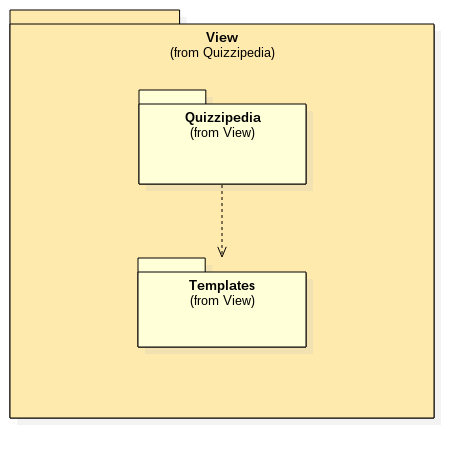
\includegraphics[scale=0.7]{../images/ViewPackage.png}
\end{center}
\end{figure}

\subsection{View::Pages}
\subsubsection{View::Pages::Page}
\begin{itemize}
\item\textbf{Funzione del componente:} rappresenta una pagina web
				\item\textbf{Relazioni d'uso con altre componenti:} L'interfaccia Page viene concretizzata dalle sue classi derivate, una rappresentativa per ogni pagina dell'applicazione\\ \\
\item\textbf{Attributi}:
	\begin{itemize}
		\item\code{- controller}: riferimento al controller della page\\
	\end{itemize}
\item\textbf{Metodi}:
	\begin{itemize}
		\item\code{+ show()}: metodo astratto che mostra il contenuto della pagina\\
	\end{itemize}
\end{itemize}

\subsubsection{View::Pages::LoginPage}
\begin{itemize}
\item\textbf{Funzione del componente:} visualizza il form di autenticazione e permette il login dell'utente. Fornisce inoltre un link alla pagina di registrazione e uno alla pagina di recupero della password 
				\item\textbf{Relazioni d'uso con altre componenti:} concretizza l'interfaccia Page da cui è diretta discendente e utilizza il template LoginForm\\ \\
La classe utilizza:
	\begin{itemize}
		\item View::Pages::Page\\
		\item View::Templates::LoginForm\\
	\end{itemize}
\item\textbf{Metodi}:
	\begin{itemize}
		\item\code{+ show()}: visualizza il form di autenticazione al sistema\\
		\textbf{Precondizioni}: viene richiesta la pagina di autenticazione. L'utente non è ancora autenticato\\
		\textbf{Postcondizioni}: viene visualizzata la pagina di autenticazione\\
	\end{itemize}
\end{itemize}

\subsubsection{View::Pages::RegistrationPage}
\begin{itemize}
\item\textbf{Funzione del componente:} visualizza il form di registrazione. Fornisce inoltre un link alla pagina di login
				\item\textbf{Relazioni d'uso con altre componenti:} concretizza l'interfaccia Page da cui è diretta discendente e utilizza il template RegistrationForm\\ \\
La classe utilizza:
	\begin{itemize}
		\item View::Pages::Page\\
		\item View::Templates::RegistrationForm\\
	\end{itemize}
\item\textbf{Metodi}:
	\begin{itemize}
		\item\code{+ show()}: visualizza il form di registrazione al sistema\\
		\textbf{Precondizioni}: viene richiesta la pagina di registrazione. L'utente non è autenticato\\
		\textbf{Postcondizioni}: viene visualizzata la pagina di registrazione\\
	\end{itemize}
\end{itemize}

\subsubsection{View::Pages::PasswordRecoveryPage}
\begin{itemize}
\item\textbf{Funzione del componente:} visualizza il form per il recupero della password
				\item\textbf{Relazioni d'uso con altre componenti:} concretizza l'interfaccia Page da cui è diretta discendente e utilizza il template PasswordRecoveryForm\\ \\
La classe utilizza:
	\begin{itemize}
		\item View::Pages::Page\\
		\item View::Templates::PasswordRecoveryForm\\
	\end{itemize}
\item\textbf{Metodi}:
	\begin{itemize}
		\item\code{+ show()}: visualizza il form per il recupero della password\\
		\textbf{Precondizioni}: viene richiesta la pagina della procedura per il recupero della password. L'utente non è autenticato\\
		\textbf{Postcondizioni}: viene visualizzata la pagina della procedura per il recupero della password\\
	\end{itemize}
\end{itemize}

\subsubsection{View::Pages::QuizCreationPage}
\begin{itemize}
\item\textbf{Funzione del componente:} visualizza il form di creazione di un nuovo questionario
				\item\textbf{Relazioni d'uso con altre componenti:} concretizza l'interfaccia Page da cui è diretta discendente e utilizza il template QuizCreationForm\\ \\
La classe utilizza:
	\begin{itemize}
		\item View::Pages::Page\\
		\item View::Templates::QuizCreationForm\\
	\end{itemize}
\item\textbf{Attributi}:
	\begin{itemize}
		\item\code{- user}: l'utente autenticato che sta creando il questionario\\
	\end{itemize}
\item\textbf{Metodi}:
	\begin{itemize}
		\item\code{+ show()}: visualizza il form per la creazione di un questionario\\
		\textbf{Precondizioni}: viene richiesta la pagina di creazione di un questionario. L'utente è autenticato\\
		\textbf{Postcondizioni}: viene visualizzata la pagina di creazione di un questionario\\
	\end{itemize}
\end{itemize}

\subsubsection{View::Pages::QuestionUpdatePage}
\begin{itemize}
\item\textbf{Funzione del componente:} visualizza il form di modifica di una domanda
				\item\textbf{Relazioni d'uso con altre componenti:} concretizza l'interfaccia Page da cui è diretta discendente e utilizza il template QuestionForm\\ \\
La classe utilizza:
	\begin{itemize}
		\item View::Pages::Page\\
		\item View::Templates::QuestionForm\\
	\end{itemize}
\item\textbf{Attributi}:
	\begin{itemize}
		\item\code{- user}: l'utente autenticato che sta modificando la domanda\\
		\item\code{- question}: la domanda da modificare\\
	\end{itemize}
\item\textbf{Metodi}:
	\begin{itemize}
		\item\code{+ show()}: visualizza il form per la modifica di una domanda compilato con i dati attuali\\
		\textbf{Precondizioni}: viene richiesta la pagina di modifica di una domanda. L'utente è autenticato\\
		\textbf{Postcondizioni}: viene visualizzata la pagina di modifica di una domanda\\
	\end{itemize}
\end{itemize}

\subsubsection{View::Pages::QuestionCreationPage}
\begin{itemize}
\item\textbf{Funzione del componente:} visualizza il form di creazione di una nuova domanda
				\item\textbf{Relazioni d'uso con altre componenti:} concretizza l'interfaccia Page da cui è diretta discendente e utilizza il template QuestionForm\\ \\
La classe utilizza:
	\begin{itemize}
		\item View::Pages::Page\\
		\item View::Templates::QuestionForm\\
	\end{itemize}
\item\textbf{Attributi}:
	\begin{itemize}
		\item\code{- user}: l'utente autenticato che sta creando la domanda\\
	\end{itemize}
\item\textbf{Metodi}:
	\begin{itemize}
		\item\code{+ show()}: visualizza il form per la creazione di una domanda\\
		\textbf{Precondizioni}: viene richiesta la pagina di creazione di una domanda. L'utente è autenticato\\
		\textbf{Postcondizioni}: viene visualizzata la pagina di creazione di una domanda\\
	\end{itemize}
\end{itemize}

\subsubsection{View::Pages::QuestionManagementPage}
\begin{itemize}
\item\textbf{Funzione del componente:} visualizza la lista delle domande create dall'utente
				\item\textbf{Relazioni d'uso con altre componenti:} concretizza l'interfaccia Page da cui è diretta discendente e utilizza il template QuestionList\\ \\
La classe utilizza:
	\begin{itemize}
		\item View::Pages::Page\\
		\item View::Templates::QuestionList\\
		\item View::Templates::Question\\
	\end{itemize}
\item\textbf{Attributi}:
	\begin{itemize}
		\item\code{- user}: l'utente autenticato che sta gestendo le proprie domande\\
		\item\code{- questions}: le domande dell'utente user\\
	\end{itemize}
\item\textbf{Metodi}:
	\begin{itemize}
		\item\code{+ show()}: visualizza la lista delle domande dell'utente permettendone la modifica e l'eliminazione. Permette inoltre di creare una nuova domanda, di ordinare la lista e fare una ricerca tra le domande\\
			\textbf{Precondizioni}: viene richiesta la pagina di gestione delle proprie domande. L'utente è autenticato\\
			\textbf{Postcondizioni}: viene visualizzata la pagina di gestione delle proprie domande\\
		\item\code{+ sort()}: ordina la lista delle domande secondo il criterio \code{by}\\
			\textbf{Precondizioni}: l'utente ha selezionato un criterio di ordinamento\\
			\textbf{Postcondizioni}: la lista di domande viene ordinata secondo il criterio inserito\\
			\textbf{Parametri}:
				\begin{itemize}
					\item\code{by}: criterio di ordinamento\\
				\end{itemize}
		\item\code{+ search()}: visualizza la lista delle domande che soddisfano il criterio di ricerca \code{query}\\
			\textbf{Precondizioni}: l'utente ha selezionato un criterio di ricerca\\
			\textbf{Postcondizioni}: la lista di domande viene filtrata secondo il criterio di ricerca\\
			\textbf{Parametri}:
				\begin{itemize}
					\item\code{query}: criterio di ricerca\\
				\end{itemize}
	\end{itemize}
\end{itemize}

\subsubsection{View::Pages::QuizResultsPage}
\begin{itemize}
\item\textbf{Funzione del componente:} visualizza i risultati del questionario appena compilato
				\item\textbf{Relazioni d'uso con altre componenti:} concretizza l'interfaccia Page da cui è diretta discendente e utilizza il template QuizResults\\ \\
La classe utilizza:
	\begin{itemize}
		\item View::Pages::Page\\
		\item View::Templates::QuizResults\\
	\end{itemize}
\item\textbf{Attributi}:
	\begin{itemize}
		\item\code{- quizResults}: i risultati del quiz appena compilato dall'utente\\
	\end{itemize}
\item\textbf{Metodi}:
	\begin{itemize}
		\item\code{+ show()}: visualizza i risultati ottenuti nel quiz appena compilato\\
		\textbf{Precondizioni}: viene richiesta la pagina di visualizzazione dei risultati di un quiz. L'utente ha compilato un quiz\\
		\textbf{Postcondizioni}: viene visualizzata la pagina di visualizzazione dei risultati di un quiz.\\
	\end{itemize}
\end{itemize}

\subsubsection{View::Pages::QuizExecutionPage}
\begin{itemize}
\item\textbf{Funzione del componente:} visualizza un questionario (una domanda alla volta) e tutti i dati relativi (tempo rimasto, numero domande, ecc...)
				\item\textbf{Relazioni d'uso con altre componenti:} concretizza l'interfaccia Page da cui è diretta discendente e utilizza il template QuestionCompilation\\ \\
La classe utilizza:
	\begin{itemize}
		\item View::Pages::Page\\
		\item View::Templates::QuestionCompilation\\
	\end{itemize}
\item\textbf{Attributi}:
	\begin{itemize}
		\item\code{- timer}: il tempo rimasto per la compilazione del questionario\\
	\end{itemize}
\item\textbf{Metodi}:
	\begin{itemize}
		\item\code{+ show()}: visualizza i dati del questionario e la domanda corrente. Permette l'inserimento o la scelta della risposta\\
			\textbf{Precondizioni}: viene richiesta la pagina di compilazione di un quiz. L'utente ha scelto un quiz\\
			\textbf{Postcondizioni}: viene visualizzata la pagina di compilazione di un quiz.\\
		\item\code{+ nextQuestion()}: visualizza la domanda successiva nel riquadro della domanda corrente\\
			\textbf{Precondizioni}: viene richiesta la domanda successiva. L'utente ha compilato la domanda corrente o ha deciso di passare alla domanda successiva\\
			\textbf{Postcondizioni}: viene visualizzata la domanda successiva.\\
		\item\code{- previousQuestion()}: visualizza la domanda precedente nel riquadro della domanda corrente\\
			\textbf{Precondizioni}: viene richiesta la domanda precedente. L'utente ha deciso di passare alla domanda precedente\\
			\textbf{Postcondizioni}: viene visualizzata la domanda precedente.\\
	\end{itemize}
\end{itemize}

\subsubsection{View::Pages::QuizListPage}
\begin{itemize}
\item\textbf{Funzione del componente:} visualizza una lista di questionari
				\item\textbf{Relazioni d'uso con altre componenti:} concretizza l'interfaccia Page da cui è diretta discendente e utilizza il template QuizList\\ \\
La classe utilizza:
	\begin{itemize}
		\item View::Pages::Page\\
		\item View::Templates::QuizList\\
		\item View::Templates::Quiz\\
	\end{itemize}
\item\textbf{Attributi}:
	\begin{itemize}
		\item\code{- quizList}: la lista di quiz da visualizzare\\
	\end{itemize}
\item\textbf{Metodi}:
	\begin{itemize}
		\item\code{+ show()}: visualizza la lista dei questionari. Permette inoltre di ordinare la lista e fare una ricerca tra i questionari\\
			\textbf{Precondizioni}: viene richiesta una pagina che mostri una lista di questionari\\
			\textbf{Postcondizioni}: viene visualizzata una pagina che mostra una lista di questionari\\
		\item\code{+ sort()}: ordina la lista dei questionari secondo il criterio \code{by}\\
			\textbf{Precondizioni}: l'utente ha selezionato un criterio di ordinamento\\
			\textbf{Postcondizioni}: la lista di questionari viene ordinata secondo il criterio inserito\\
			\textbf{Parametri}:
				\begin{itemize}
					\item\code{by}: criterio di ordinamento\\
				\end{itemize}
		\item\code{+ search()}: visualizza la lista dei questionari che soddisfano il criterio di ricerca \code{query}\\
			\textbf{Precondizioni}: l'utente ha selezionato un criterio di ricerca\\
			\textbf{Postcondizioni}: la lista dei questionari viene filtrata secondo il criterio di ricerca\\
			\textbf{Parametri}:
				\begin{itemize}
					\item\code{query}: criterio di ricerca\\
				\end{itemize}
	\end{itemize}
\end{itemize}

\subsubsection{View::Pages::CategoryListPage}
\begin{itemize}
\item\textbf{Funzione del componente:} visualizza la lista delle categorie
				\item\textbf{Relazioni d'uso con altre componenti:} concretizza l'interfaccia Page da cui è diretta discendente\\ \\
La classe utilizza:
	\begin{itemize}
		\item View::Pages::Page\\
	\end{itemize}
\item\textbf{Attributi}:
	\begin{itemize}
		\item\code{- categories}: la lista delle categorie da visualizzare\\
	\end{itemize}
\item\textbf{Metodi}:
	\begin{itemize}
		\item\code{+ show()}: visualizza la lista delle categorie. Permette inoltre di ordinare la lista e fare una ricerca tra le categorie\\
			\textbf{Precondizioni}: viene richiesta una pagina che mostri una lista di categorie\\
			\textbf{Postcondizioni}: viene visualizzata una pagina che mostra una lista di categorie\\
		\item\code{+ sort(by)}: ordina la lista delle categorie secondo il criterio \code{by}\\
			\textbf{Precondizioni}: l'utente ha selezionato un criterio di ordinamento\\
			\textbf{Postcondizioni}: la lista di categorie viene ordinata secondo il criterio inserito\\
			\textbf{Parametri}:
				\begin{itemize}
					\item\code{by}: criterio di ordinamento\\
				\end{itemize}
		\item\code{+ search()}: visualizza la lista delle categorie che soddisfano il criterio di ricerca \code{query}\\
			\textbf{Precondizioni}: l'utente ha selezionato un criterio di ricerca\\
			\textbf{Postcondizioni}: la lista delle categorie viene filtrata secondo il criterio di ricerca\\
			\textbf{Parametri}:
				\begin{itemize}
					\item\code{query}: criterio di ricerca\\
				\end{itemize}
	\end{itemize}
\end{itemize}

\subsection{View::Templates}
\subsubsection{View::Templates::QuestionList}
\begin{itemize}
\item\textbf{Funzione del componente:} visualizza una lista di domande
				\item\textbf{Relazioni d'uso con altre componenti:} composta da Question\\ \\
La classe utilizza:
	\begin{itemize}
		\item
	\end{itemize}
\item\textbf{Attributi}:
\begin{itemize}
		\item\code{}\\
		\item\code{}\\
		\item\code{}\\
		\item\code{}\\
	\end{itemize}
\item\textbf{Metodi}:
	\begin{itemize}
		\item\code{}\\
		\textbf{Parametri}:
			\begin{itemize}
		\item\code{}\\
			\end{itemize}
		\item\code{}\\
		\textbf{Parametri}:
			\begin{itemize}
				\item\code{}\\
		\end{itemize}
		\item\code{}\\
		\textbf{Parametri}:
			\begin{itemize}
				\item\code{}\\
			\end{itemize}
		\item\code{}\\
		\textbf{Parametri}:
			\begin{itemize}
				\item\code{}\\
			\end{itemize}
	\end{itemize}
\end{itemize}

\subsubsection{View::Templates::Question}
\begin{itemize}
\item\textbf{Funzione del componente:} visualizza una domanda inserita in una lista
				\item\textbf{Relazioni d'uso con altre componenti:} usata solo da QuestionList per creare la sta\\\
La classe utilizza:
\begin{itemize}
		\item
	\end{itemize}
\item\textbf{Attributi}:
	\begin{itemize}
		\item\code{}\\
		\item\code{}\\
		\item\code{}\\
	\item\code{}\\
	\end{itemize}
\item\textbf{Metodi}:
\begin{itemize}
		\item\code{}\\
		\textbf{Parametri}:
			\begin{itemize}
			\item\code{}\\
			\end{itemize}
		\item\code{}\\
		\textbf{Parametri}:
			\begin{itemize}
				\item\code{}\\
			\end{itemize}
		\item\code{}\\
		\textbf{Parametri}:
			\begin{itemize}
				\item\code{}\\
			\end{itemize}
		\item\code{}\\
		\textbf{Parametri}:
			\begin{itemize}
				\item\code{}\\
			\end{itemize}
	\end{itemize}
\end{itemize}

\subsubsection{View::Templates::QuizList}
\begin{itemize}
\item\textbf{Funzione del componente:} visualizza una lista di quiz
				\item\textbf{Relazioni d'uso con altre componenti:} composta da Quiz\\ \\
La classe utilizza:
	\begin{itemize}
		\item
	\end{itemize}
\item\textbf{Attributi}:
	\begin{itemize}
		\item\code{}\\
		\item\code{}\\
		\item\code{}\\
		\item\code{}\\
	\end{itemize}
\item\textbf{Metodi}:
	\begin{itemize}
		\item\code{}\\
	\textbf{Parametri}:
			\begin{itemize}
				\item\code{}\\
			\end{itemize}
		\item\code{}\\
		\textbf{Parametri}:
			\begin{itemize}
				\item\code{}\\
			\end{itemize}
		\item\code{}\\
		\textbf{Parametri}:
			\begin{itemize}
				\item\code{}\\
			\end{itemize}
		\item\code{}\\
		\textbf{Parametri}:
			\begin{itemize}
				\item\code{}\\
			\end{itemize}
	\end{itemize}
\end{itemize}

\subsubsection{View::Templates::Quiz}
\begin{itemize}
\item\textbf{Funzione del componente:} visualizza un quiz inserito in una lista
				\item\textbf{Relazioni d'uso con altre componenti:} usata solo da QuizList per creare la lista\\ \\
 -La classe utilizza:
 -	\begin{itemize}
 		\item
 	\end{itemize}
 \item\textbf{Attributi}:
 	\begin{itemize}
 		\item\code{}\\
 		\item\code{}\\
 		\item\code{}\\
 		\item\code{}\\
 	\end{itemize}
 \item\textbf{Metodi}:
 	\begin{itemize}
 		\item\code{}\\
 		\textbf{Parametri}:
 			\begin{itemize}
 				\item\code{}\\
 			\end{itemize}
 		\item\code{}\\
 		\textbf{Parametri}:
 			\begin{itemize}
 				\item\code{}\\
 			\end{itemize}
 		\item\code{}\\
 		\textbf{Parametri}:
 			\begin{itemize}
 				\item\code{}\\
 			\end{itemize}
 		\item\code{}\\
 		\textbf{Parametri}:
 			\begin{itemize}
 				\item\code{}\\
 			\end{itemize}
 	\end{itemize}
 \end{itemize}
 
 \subsubsection{View::Templates::QuestionForm}
 \begin{itemize}
 \item\textbf{Funzione del componente:} visualizza il form per i dati di una domanda. Utilizzabile sia per la creazione che per la modifica della domanda (se viene modificata una domanda già esistente nei campi vengono inseriti i valori attuali)
 \item\textbf{Relazioni con altre componenti}\\
 La classe utilizza:
 	\begin{itemize}
 		\item
 	\end{itemize}
 \item\textbf{Attributi}:
 	\begin{itemize}
 		\item\code{}\\
 		\item\code{}\\
 		\item\code{}\\
 		\item\code{}\\
 	\end{itemize}
 \item\textbf{Metodi}:
 	\begin{itemize}
 		\item\code{}\\
 		\textbf{Parametri}:
 			\begin{itemize}
 				\item\code{}\\
 			\end{itemize}
 		\item\code{}\\
 		\textbf{Parametri}:
 			\begin{itemize}
 				\item\code{}\\
 			\end{itemize}
 		\item\code{}\\
 		\textbf{Parametri}:
 			\begin{itemize}
 				\item\code{}\\
 			\end{itemize}
 		\item\code{}\\
 		\textbf{Parametri}:
 			\begin{itemize}
 				\item\code{}\\
 			\end{itemize}
 	\end{itemize}
 \end{itemize}
 
 \subsubsection{View::Templates::QuizCreationForm}
 \begin{itemize}
 \item\textbf{Funzione del componente:} visualizza il form di creazione di un questionario
 \item\textbf{Relazioni con altre componenti}\\
 La classe utilizza:
 	\begin{itemize}
 		\item
 	\end{itemize}
 \item\textbf{Attributi}:
 	\begin{itemize}
 		\item\code{}\\
 		\item\code{}\\
 		\item\code{}\\
 		\item\code{}\\
 	\end{itemize}
 \item\textbf{Metodi}:
 	\begin{itemize}
 		\item\code{}\\
 		\textbf{Parametri}:
 			\begin{itemize}
 				\item\code{}\\
 			\end{itemize}
 		\item\code{}\\
 		\textbf{Parametri}:
 			\begin{itemize}
 				\item\code{}\\
 			\end{itemize}
 		\item\code{}\\
 		\textbf{Parametri}:
 			\begin{itemize}
 				\item\code{}\\
 			\end{itemize}
 		\item\code{}\\
 		\textbf{Parametri}:
 			\begin{itemize}
 				\item\code{}\\
 			\end{itemize}
 	\end{itemize}
 \end{itemize}
 
 \subsubsection{View::Templates::QuestionCompilation}
 \begin{itemize}
 \item\textbf{Funzione del componente:} visualizza una domanda e ne permette la compilazione
 \item\textbf{Relazioni con altre componenti}\\
 La classe utilizza:
 	\begin{itemize}
 		\item
 	\end{itemize}
 \item\textbf{Attributi}:
 	\begin{itemize}
 		\item\code{}\\
 		\item\code{}\\
 		\item\code{}\\
 		\item\code{}\\
 	\end{itemize}
 \item\textbf{Metodi}:
 	\begin{itemize}
 		\item\code{}\\
 		\textbf{Parametri}:
 			\begin{itemize}
 				\item\code{}\\
 			\end{itemize}
 		\item\code{}\\
 		\textbf{Parametri}:
 			\begin{itemize}
 				\item\code{}\\
 			\end{itemize}
 		\item\code{}\\
 		\textbf{Parametri}:
 			\begin{itemize}
 				\item\code{}\\
 			\end{itemize}
 		\item\code{}\\
 		\textbf{Parametri}:
 			\begin{itemize}
 				\item\code{}\\
 			\end{itemize}
 	\end{itemize}
 \end{itemize}
 
 \subsubsection{View::Templates::QuizResults}
 \begin{itemize}
 \item\textbf{Funzione del componente:} visualizza i risultati ottenuti in seguito alla compilazione di un quiz
 \item\textbf{Relazioni con altre componenti}\\
 La classe utilizza:
 	\begin{itemize}
 		\item
 	\end{itemize}
 \item\textbf{Attributi}:
 	\begin{itemize}
 		\item\code{}\\
 		\item\code{}\\
 		\item\code{}\\
 		\item\code{}\\
 	\end{itemize}
 \item\textbf{Metodi}:
 	\begin{itemize}
 		\item\code{}\\
 		\textbf{Parametri}:
 			\begin{itemize}
 				\item\code{}\\
 			\end{itemize}
 		\item\code{}\\
 		\textbf{Parametri}:
 			\begin{itemize}
 				\item\code{}\\
 			\end{itemize}
 		\item\code{}\\
 		\textbf{Parametri}:
 			\begin{itemize}
 				\item\code{}\\
 			\end{itemize}
 		\item\code{}\\
 		\textbf{Parametri}:
 			\begin{itemize}
 				\item\code{}\\
 			\end{itemize}
 	\end{itemize}
 \end{itemize}
 
 \subsubsection{View::Templates::RegistrationForm}
 \begin{itemize}
 \item\textbf{Funzione del componente:} visualizza un form per la registrazione di un nuovo utente
 \item\textbf{Relazioni con altre componenti}\\
 La classe utilizza:
 	\begin{itemize}
 		\item
 	\end{itemize}
 \item\textbf{Attributi}:
 	\begin{itemize}
 		\item\code{}\\
 		\item\code{}\\
 		\item\code{}\\
 		\item\code{}\\
 	\end{itemize}
 \item\textbf{Metodi}:
 	\begin{itemize}
 		\item\code{}\\
 		\textbf{Parametri}:
 			\begin{itemize}
 				\item\code{}\\
 			\end{itemize}
 		\item\code{}\\
 		\textbf{Parametri}:
 			\begin{itemize}
 				\item\code{}\\
 			\end{itemize}
 		\item\code{}\\
 		\textbf{Parametri}:
 			\begin{itemize}
 				\item\code{}\\
 			\end{itemize}
 		\item\code{}\\
 		\textbf{Parametri}:
 			\begin{itemize}
 				\item\code{}\\
 			\end{itemize}
 	\end{itemize}
 \end{itemize}
 
 \subsubsection{View::Templates::LoginForm}
 \begin{itemize}
 \item\textbf{Funzione del componente:} visualizza un form per l'autenticazione di un utente
 \item\textbf{Relazioni con altre componenti}\\
 La classe utilizza:
 	\begin{itemize}
 		\item
 	\end{itemize}
 \item\textbf{Attributi}:
 	\begin{itemize}
 		\item\code{}\\
 		\item\code{}\\
 		\item\code{}\\
 		\item\code{}\\
 	\end{itemize}
 \item\textbf{Metodi}:
 	\begin{itemize}
 		\item\code{}\\
 		\textbf{Parametri}:
 			\begin{itemize}
 				\item\code{}\\
 			\end{itemize}
 		\item\code{}\\
 		\textbf{Parametri}:
 			\begin{itemize}
 				\item\code{}\\
 			\end{itemize}
 		\item\code{}\\
 		\textbf{Parametri}:
 			\begin{itemize}
 				\item\code{}\\
 			\end{itemize}
 		\item\code{}\\
 		\textbf{Parametri}:
 			\begin{itemize}
 				\item\code{}\\
 			\end{itemize}
 	\end{itemize}
 \end{itemize}
 
 \subsubsection{View::Templates::PasswordRecoveryForm}
 \begin{itemize}
 \item\textbf{Funzione del componente:} visualizza un form per il recupero della password dimenticata
 \item\textbf{Relazioni con altre componenti}\\
 La classe utilizza:
 	\begin{itemize}
 		\item
 	\end{itemize}
 \item\textbf{Attributi}:
 	\begin{itemize}
 		\item\code{}\\
 		\item\code{}\\
 		\item\code{}\\
 		\item\code{}\\
 	\end{itemize}
 \item\textbf{Metodi}:
 	\begin{itemize}
 		\item\code{}\\
 		\textbf{Parametri}:
 			\begin{itemize}
 				\item\code{}\\
 			\end{itemize}
 		\item\code{}\\
 		\textbf{Parametri}:
 			\begin{itemize}
 				\item\code{}\\
 			\end{itemize}
 		\item\code{}\\
 		\textbf{Parametri}:
 			\begin{itemize}
 				\item\code{}\\
 			\end{itemize}
 		\item\code{}\\
 		\textbf{Parametri}:
 			\begin{itemize}
 				\item\code{}\\
 			\end{itemize}
 	\end{itemize}
 \end{itemize}
 
 \subsubsection{View::Templates::SearchForm}
 \begin{itemize}
 \item\textbf{Funzione del componente:}
 \item\textbf{Relazioni con altre componenti}\\
 La classe utilizza:
 	\begin{itemize}
 		\item
 	\end{itemize}
 \item\textbf{Attributi}:
 	\begin{itemize}
 		\item\code{}\\
 		\item\code{}\\
 		\item\code{}\\
 		\item\code{}\\
 	\end{itemize}
 \item\textbf{Metodi}:
 	\begin{itemize}
 		\item\code{}\\
 		\textbf{Parametri}:
 			\begin{itemize}
 				\item\code{}\\
 			\end{itemize}
 		\item\code{}\\
 		\textbf{Parametri}:
 			\begin{itemize}
 				\item\code{}\\
 			\end{itemize}
 		\item\code{}\\
 		\textbf{Parametri}:
 			\begin{itemize}
 				\item\code{}\\
 			\end{itemize}
 		\item\code{}\\
 		\textbf{Parametri}:
 			\begin{itemize}
 				\item\code{}\\
 			\end{itemize}
 	\end{itemize}
 \end{itemize}
	\newpage
	\section{Package Model}\begin{figure}[h!]
\begin{center}
	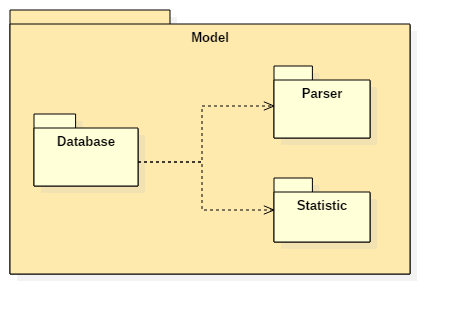
\includegraphics[scale=0.7]{../images/ModelPackage.png}
\end{center}
\end{figure}
\subsection{Model::Database}
\subsubsection{Model::Database::UserManager}
\begin{itemize}
\item\textbf{Funzione}:
\item\textbf{Relazioni con altre componenti}\\
La classe utilizza:
	\begin{itemize}
		\item
	\end{itemize}
\item\textbf{Attributi}:
	\begin{itemize}
		\item\code{}\\
		\item\code{}\\
		\item\code{}\\
		\item\code{}\\
	\end{itemize}
\item\textbf{Metodi}:
	\begin{itemize}
		\item\code{}\\
		\textbf{Parametri}:
			\begin{itemize}
				\item\code{}\\
			\end{itemize}
		\item\code{}\\
		\textbf{Parametri}:
			\begin{itemize}
				\item\code{}\\
			\end{itemize}
		\item\code{}\\
		\textbf{Parametri}:
			\begin{itemize}
				\item\code{}\\
			\end{itemize}
		\item\code{}\\
		\textbf{Parametri}:
			\begin{itemize}
				\item\code{}\\
			\end{itemize}
	\end{itemize}
\end{itemize}

\subsubsection{Model::Database::QuizManager}
\begin{itemize}
\item\textbf{Funzione}:
\item\textbf{Relazioni con altre componenti}\\
La classe utilizza:
	\begin{itemize}
		\item
	\end{itemize}
\item\textbf{Attributi}:
	\begin{itemize}
		\item\code{}\\
		\item\code{}\\
		\item\code{}\\
		\item\code{}\\
	\end{itemize}
\item\textbf{Metodi}:
	\begin{itemize}
		\item\code{}\\
		\textbf{Parametri}:
			\begin{itemize}
				\item\code{}\\
			\end{itemize}
		\item\code{}\\
		\textbf{Parametri}:
			\begin{itemize}
				\item\code{}\\
			\end{itemize}
		\item\code{}\\
		\textbf{Parametri}:
			\begin{itemize}
				\item\code{}\\
			\end{itemize}
		\item\code{}\\
		\textbf{Parametri}:
			\begin{itemize}
				\item\code{}\\
			\end{itemize}
	\end{itemize}
\end{itemize}

\subsubsection{Model::Database::QuestionManager}
\begin{itemize}
\item\textbf{Funzione}:
\item\textbf{Relazioni con altre componenti}\\
La classe utilizza:
	\begin{itemize}
		\item
	\end{itemize}
\item\textbf{Attributi}:
	\begin{itemize}
		\item\code{}\\
		\item\code{}\\
		\item\code{}\\
		\item\code{}\\
	\end{itemize}
\item\textbf{Metodi}:
	\begin{itemize}
		\item\code{}\\
		\textbf{Parametri}:
			\begin{itemize}
				\item\code{}\\
			\end{itemize}
		\item\code{}\\
		\textbf{Parametri}:
			\begin{itemize}
				\item\code{}\\
			\end{itemize}
		\item\code{}\\
		\textbf{Parametri}:
			\begin{itemize}
				\item\code{}\\
			\end{itemize}
		\item\code{}\\
		\textbf{Parametri}:
			\begin{itemize}
				\item\code{}\\
			\end{itemize}
	\end{itemize}
\end{itemize}

\subsection{Model::Parser}
\subsubsection{Model::Parser::Parser}
\begin{itemize}
\item\textbf{Funzione}:
\item\textbf{Relazioni con altre componenti}\\
La classe utilizza:
	\begin{itemize}
		\item
	\end{itemize}
\item\textbf{Attributi}:
	\begin{itemize}
		\item\code{}\\
		\item\code{}\\
		\item\code{}\\
		\item\code{}\\
	\end{itemize}
\item\textbf{Metodi}:
	\begin{itemize}
		\item\code{}\\
		\textbf{Parametri}:
			\begin{itemize}
				\item\code{}\\
			\end{itemize}
		\item\code{}\\
		\textbf{Parametri}:
			\begin{itemize}
				\item\code{}\\
			\end{itemize}
		\item\code{}\\
		\textbf{Parametri}:
			\begin{itemize}
				\item\code{}\\
			\end{itemize}
		\item\code{}\\
		\textbf{Parametri}:
			\begin{itemize}
				\item\code{}\\
			\end{itemize}
	\end{itemize}
\end{itemize}

\subsection{Model::Statistics}
\subsubsection{Model::Statistics::Statistics}
\begin{itemize}
\item\textbf{Funzione}:
\item\textbf{Relazioni con altre componenti}\\
La classe utilizza:
	\begin{itemize}
		\item
	\end{itemize}
\item\textbf{Attributi}:
	\begin{itemize}
		\item\code{}\\
		\item\code{}\\
		\item\code{}\\
		\item\code{}\\
	\end{itemize}
\item\textbf{Metodi}:
	\begin{itemize}
		\item\code{}\\
		\textbf{Parametri}:
			\begin{itemize}
				\item\code{}\\
			\end{itemize}
		\item\code{}\\
		\textbf{Parametri}:
			\begin{itemize}
				\item\code{}\\
			\end{itemize}
		\item\code{}\\
		\textbf{Parametri}:
			\begin{itemize}
				\item\code{}\\
			\end{itemize}
		\item\code{}\\
		\textbf{Parametri}:
			\begin{itemize}
				\item\code{}\\
			\end{itemize}
	\end{itemize}
\end{itemize}

\subsection{Model::Publishers}
\subsubsection{Model::Publishers::UserPublishers}
\begin{itemize}
\item\textbf{Funzione}:
\item\textbf{Relazioni con altre componenti}\\
La classe utilizza:
	\begin{itemize}
		\item
	\end{itemize}
\item\textbf{Attributi}:
	\begin{itemize}
		\item\code{}\\
		\item\code{}\\
		\item\code{}\\
		\item\code{}\\
	\end{itemize}
\item\textbf{Metodi}:
	\begin{itemize}
		\item\code{}\\
		\textbf{Parametri}:
			\begin{itemize}
				\item\code{}\\
			\end{itemize}
		\item\code{}\\
		\textbf{Parametri}:
			\begin{itemize}
				\item\code{}\\
			\end{itemize}
		\item\code{}\\
		\textbf{Parametri}:
			\begin{itemize}
				\item\code{}\\
			\end{itemize}
		\item\code{}\\
		\textbf{Parametri}:
			\begin{itemize}
				\item\code{}\\
			\end{itemize}
	\end{itemize}
\end{itemize}

\subsubsection{Model::Publishers::QuizPublishers}
\begin{itemize}
\item\textbf{Funzione}:
\item\textbf{Relazioni con altre componenti}\\
La classe utilizza:
	\begin{itemize}
		\item
	\end{itemize}
\item\textbf{Attributi}:
	\begin{itemize}
		\item\code{}\\
		\item\code{}\\
		\item\code{}\\
		\item\code{}\\
	\end{itemize}
\item\textbf{Metodi}:
	\begin{itemize}
		\item\code{}\\
		\textbf{Parametri}:
			\begin{itemize}
				\item\code{}\\
			\end{itemize}
		\item\code{}\\
		\textbf{Parametri}:
			\begin{itemize}
				\item\code{}\\
			\end{itemize}
		\item\code{}\\
		\textbf{Parametri}:
			\begin{itemize}
				\item\code{}\\
			\end{itemize}
		\item\code{}\\
		\textbf{Parametri}:
			\begin{itemize}
				\item\code{}\\
			\end{itemize}
	\end{itemize}
\end{itemize}

\subsubsection{Model::Publishers::QuestionPublishers}
\begin{itemize}
\item\textbf{Funzione}:
\item\textbf{Relazioni con altre componenti}\\
La classe utilizza:
	\begin{itemize}
		\item
	\end{itemize}
\item\textbf{Attributi}:
	\begin{itemize}
		\item\code{}\\
		\item\code{}\\
		\item\code{}\\
		\item\code{}\\
	\end{itemize}
\item\textbf{Metodi}:
	\begin{itemize}
		\item\code{}\\
		\textbf{Parametri}:
			\begin{itemize}
				\item\code{}\\
			\end{itemize}
		\item\code{}\\
		\textbf{Parametri}:
			\begin{itemize}
				\item\code{}\\
			\end{itemize}
		\item\code{}\\
		\textbf{Parametri}:
			\begin{itemize}
				\item\code{}\\
			\end{itemize}
		\item\code{}\\
		\textbf{Parametri}:
			\begin{itemize}
				\item\code{}\\
			\end{itemize}
	\end{itemize}
\end{itemize}
	\newpage
	\section{Package Presenter}
\begin{figure}[h!]
\begin{center}
	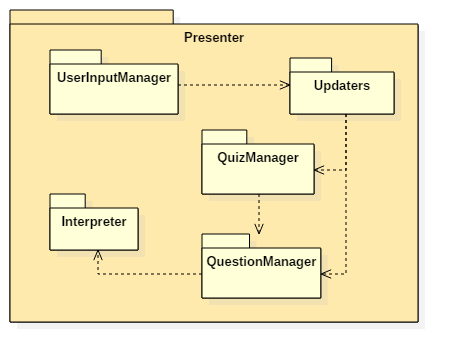
\includegraphics[scale=0.7]{../images/PresenterPackage.png}
\end{center}
\end{figure}
\subsection{Presenter::UserInputManager}
\subsubsection{Presenter::UserInputManager::InputManager}
\begin{itemize}
\item\textbf{Funzione}:
\item\textbf{Relazioni con altre componenti}\\
La classe utilizza:
	\begin{itemize}
		\item
	\end{itemize}
\item\textbf{Attributi}:
	\begin{itemize}
		\item\code{}\\
		\item\code{}\\
		\item\code{}\\
		\item\code{}\\
	\end{itemize}
\item\textbf{Metodi}:
	\begin{itemize}
		\item\code{}\\
		\textbf{Parametri}:
			\begin{itemize}
				\item\code{}\\
			\end{itemize}
		\item\code{}\\
		\textbf{Parametri}:
			\begin{itemize}
				\item\code{}\\
			\end{itemize}
		\item\code{}\\
		\textbf{Parametri}:
			\begin{itemize}
				\item\code{}\\
			\end{itemize}
		\item\code{}\\
		\textbf{Parametri}:
			\begin{itemize}
				\item\code{}\\
			\end{itemize}
	\end{itemize}
\end{itemize}

\subsubsection{Presenter::UserInputManager::Input}
\begin{itemize}
\item\textbf{Funzione}:
\item\textbf{Relazioni con altre componenti}\\
La classe utilizza:
	\begin{itemize}
		\item
	\end{itemize}
\item\textbf{Attributi}:
	\begin{itemize}
		\item\code{}\\
		\item\code{}\\
		\item\code{}\\
		\item\code{}\\
	\end{itemize}
\item\textbf{Metodi}:
	\begin{itemize}
		\item\code{}\\
		\textbf{Parametri}:
			\begin{itemize}
				\item\code{}\\
			\end{itemize}
		\item\code{}\\
		\textbf{Parametri}:
			\begin{itemize}
				\item\code{}\\
			\end{itemize}
		\item\code{}\\
		\textbf{Parametri}:
			\begin{itemize}
				\item\code{}\\
			\end{itemize}
		\item\code{}\\
		\textbf{Parametri}:
			\begin{itemize}
				\item\code{}\\
			\end{itemize}
	\end{itemize}
\end{itemize}

\subsubsection{Presenter::UserInputManager::CreateQuiz}
\begin{itemize}
\item\textbf{Funzione}:
\item\textbf{Relazioni con altre componenti}\\
La classe utilizza:
	\begin{itemize}
		\item
	\end{itemize}
\item\textbf{Attributi}:
	\begin{itemize}
		\item\code{}\\
		\item\code{}\\
		\item\code{}\\
		\item\code{}\\
	\end{itemize}
\item\textbf{Metodi}:
	\begin{itemize}
		\item\code{}\\
		\textbf{Parametri}:
			\begin{itemize}
				\item\code{}\\
			\end{itemize}
		\item\code{}\\
		\textbf{Parametri}:
			\begin{itemize}
				\item\code{}\\
			\end{itemize}
		\item\code{}\\
		\textbf{Parametri}:
			\begin{itemize}
				\item\code{}\\
			\end{itemize}
		\item\code{}\\
		\textbf{Parametri}:
			\begin{itemize}
				\item\code{}\\
			\end{itemize}
	\end{itemize}
\end{itemize}

\subsubsection{Presenter::UserInputManager::AddQuestion}\begin{itemize}
\item\textbf{Funzione}:
\item\textbf{Relazioni con altre componenti}\\
La classe utilizza:
	\begin{itemize}
		\item
	\end{itemize}
\item\textbf{Attributi}:
	\begin{itemize}
		\item\code{}\\
		\item\code{}\\
		\item\code{}\\
		\item\code{}\\
	\end{itemize}
\item\textbf{Metodi}:
	\begin{itemize}
		\item\code{}\\
		\textbf{Parametri}:
			\begin{itemize}
				\item\code{}\\
			\end{itemize}
		\item\code{}\\
		\textbf{Parametri}:
			\begin{itemize}
				\item\code{}\\
			\end{itemize}
		\item\code{}\\
		\textbf{Parametri}:
			\begin{itemize}
				\item\code{}\\
			\end{itemize}
		\item\code{}\\
		\textbf{Parametri}:
			\begin{itemize}
				\item\code{}\\
			\end{itemize}
	\end{itemize}
\end{itemize}

\subsubsection{Presenter::UserInputManager::RemoveQuestion}
\begin{itemize}
\item\textbf{Funzione}:
\item\textbf{Relazioni con altre componenti}\\
La classe utilizza:
	\begin{itemize}
		\item
	\end{itemize}
\item\textbf{Attributi}:
	\begin{itemize}
		\item\code{}\\
		\item\code{}\\
		\item\code{}\\
		\item\code{}\\
	\end{itemize}
\item\textbf{Metodi}:
	\begin{itemize}
		\item\code{}\\
		\textbf{Parametri}:
			\begin{itemize}
				\item\code{}\\
			\end{itemize}
		\item\code{}\\
		\textbf{Parametri}:
			\begin{itemize}
				\item\code{}\\
			\end{itemize}
		\item\code{}\\
		\textbf{Parametri}:
			\begin{itemize}
				\item\code{}\\
			\end{itemize}
		\item\code{}\\
		\textbf{Parametri}:
			\begin{itemize}
				\item\code{}\\
			\end{itemize}
	\end{itemize}
\end{itemize}

\subsubsection{Presenter::UserInputManager::SaveQuiz}
\begin{itemize}
\item\textbf{Funzione}:
\item\textbf{Relazioni con altre componenti}\\
La classe utilizza:
	\begin{itemize}
		\item
	\end{itemize}
\item\textbf{Attributi}:
	\begin{itemize}
		\item\code{}\\
		\item\code{}\\
		\item\code{}\\
		\item\code{}\\
	\end{itemize}
\item\textbf{Metodi}:
	\begin{itemize}
		\item\code{}\\
		\textbf{Parametri}:
			\begin{itemize}
				\item\code{}\\
			\end{itemize}
		\item\code{}\\
		\textbf{Parametri}:
			\begin{itemize}
				\item\code{}\\
			\end{itemize}
		\item\code{}\\
		\textbf{Parametri}:
			\begin{itemize}
				\item\code{}\\
			\end{itemize}
		\item\code{}\\
		\textbf{Parametri}:
			\begin{itemize}
				\item\code{}\\
			\end{itemize}
	\end{itemize}
\end{itemize}

\subsubsection{Presenter::UserInputManager::CreateQuestion}
\begin{itemize}
\item\textbf{Funzione}:
\item\textbf{Relazioni con altre componenti}\\
La classe utilizza:
	\begin{itemize}
		\item
	\end{itemize}
\item\textbf{Attributi}:
	\begin{itemize}
		\item\code{}\\
		\item\code{}\\
		\item\code{}\\
		\item\code{}\\
	\end{itemize}
\item\textbf{Metodi}:
	\begin{itemize}
		\item\code{}\\
		\textbf{Parametri}:
			\begin{itemize}
				\item\code{}\\
			\end{itemize}
		\item\code{}\\
		\textbf{Parametri}:
			\begin{itemize}
				\item\code{}\\
			\end{itemize}
		\item\code{}\\
		\textbf{Parametri}:
			\begin{itemize}
				\item\code{}\\
			\end{itemize}
		\item\code{}\\
		\textbf{Parametri}:
			\begin{itemize}
				\item\code{}\\
			\end{itemize}
	\end{itemize}
\end{itemize}

\subsubsection{Presenter::UserInputManager::SaveQuestion}
\begin{itemize}
\item\textbf{Funzione}:
\item\textbf{Relazioni con altre componenti}\\
La classe utilizza:
	\begin{itemize}
		\item
	\end{itemize}
\item\textbf{Attributi}:
	\begin{itemize}
		\item\code{}\\
		\item\code{}\\
		\item\code{}\\
		\item\code{}\\
	\end{itemize}
\item\textbf{Metodi}:
	\begin{itemize}
		\item\code{}\\
		\textbf{Parametri}:
			\begin{itemize}
				\item\code{}\\
			\end{itemize}
		\item\code{}\\
		\textbf{Parametri}:
			\begin{itemize}
				\item\code{}\\
			\end{itemize}
		\item\code{}\\
		\textbf{Parametri}:
			\begin{itemize}
				\item\code{}\\
			\end{itemize}
		\item\code{}\\
		\textbf{Parametri}:
			\begin{itemize}
				\item\code{}\\
			\end{itemize}
	\end{itemize}
\end{itemize}

\subsubsection{Presenter::UserInputManager::DeleteQuestion}
\begin{itemize}
\item\textbf{Funzione}:
\item\textbf{Relazioni con altre componenti}\\
La classe utilizza:
	\begin{itemize}
		\item
	\end{itemize}
\item\textbf{Attributi}:
	\begin{itemize}
		\item\code{}\\
		\item\code{}\\
		\item\code{}\\
		\item\code{}\\
	\end{itemize}
\item\textbf{Metodi}:
	\begin{itemize}
		\item\code{}\\
		\textbf{Parametri}:
			\begin{itemize}
				\item\code{}\\
			\end{itemize}
		\item\code{}\\
		\textbf{Parametri}:
			\begin{itemize}
				\item\code{}\\
			\end{itemize}
		\item\code{}\\
		\textbf{Parametri}:
			\begin{itemize}
				\item\code{}\\
			\end{itemize}
		\item\code{}\\
		\textbf{Parametri}:
			\begin{itemize}
				\item\code{}\\
			\end{itemize}
	\end{itemize}
\end{itemize}

\subsubsection{Presenter::UserInputManager::ChooseQuiz}
\begin{itemize}
\item\textbf{Funzione}:
\item\textbf{Relazioni con altre componenti}\\
La classe utilizza:
	\begin{itemize}
		\item
	\end{itemize}
\item\textbf{Attributi}:
	\begin{itemize}
		\item\code{}\\
		\item\code{}\\
		\item\code{}\\
		\item\code{}\\
	\end{itemize}
\item\textbf{Metodi}:
	\begin{itemize}
		\item\code{}\\
		\textbf{Parametri}:
			\begin{itemize}
				\item\code{}\\
			\end{itemize}
		\item\code{}\\
		\textbf{Parametri}:
			\begin{itemize}
				\item\code{}\\
			\end{itemize}
		\item\code{}\\
		\textbf{Parametri}:
			\begin{itemize}
				\item\code{}\\
			\end{itemize}
		\item\code{}\\
		\textbf{Parametri}:
			\begin{itemize}
				\item\code{}\\
			\end{itemize}
	\end{itemize}
\end{itemize}

\subsubsection{Presenter::UserInputManager::StartQuiz}
\begin{itemize}
\item\textbf{Funzione}:
\item\textbf{Relazioni con altre componenti}\\
La classe utilizza:
	\begin{itemize}
		\item
	\end{itemize}
\item\textbf{Attributi}:
	\begin{itemize}
		\item\code{}\\
		\item\code{}\\
		\item\code{}\\
		\item\code{}\\
	\end{itemize}
\item\textbf{Metodi}:
	\begin{itemize}
		\item\code{}\\
		\textbf{Parametri}:
			\begin{itemize}
				\item\code{}\\
			\end{itemize}
		\item\code{}\\
		\textbf{Parametri}:
			\begin{itemize}
				\item\code{}\\
			\end{itemize}
		\item\code{}\\
		\textbf{Parametri}:
			\begin{itemize}
				\item\code{}\\
			\end{itemize}
		\item\code{}\\
		\textbf{Parametri}:
			\begin{itemize}
				\item\code{}\\
			\end{itemize}
	\end{itemize}
\end{itemize}

\subsubsection{Presenter::UserInputManager::NextQuestion}
\begin{itemize}
\item\textbf{Funzione}:
\item\textbf{Relazioni con altre componenti}\\
La classe utilizza:
	\begin{itemize}
		\item
	\end{itemize}
\item\textbf{Attributi}:
	\begin{itemize}
		\item\code{}\\
		\item\code{}\\
		\item\code{}\\
		\item\code{}\\
	\end{itemize}
\item\textbf{Metodi}:
	\begin{itemize}
		\item\code{}\\
		\textbf{Parametri}:
			\begin{itemize}
				\item\code{}\\
			\end{itemize}
		\item\code{}\\
		\textbf{Parametri}:
			\begin{itemize}
				\item\code{}\\
			\end{itemize}
		\item\code{}\\
		\textbf{Parametri}:
			\begin{itemize}
				\item\code{}\\
			\end{itemize}
		\item\code{}\\
		\textbf{Parametri}:
			\begin{itemize}
				\item\code{}\\
			\end{itemize}
	\end{itemize}
\end{itemize}

\subsubsection{Presenter::UserInputManager::PreviousQuestion}
\begin{itemize}
\item\textbf{Funzione}:
\item\textbf{Relazioni con altre componenti}\\
La classe utilizza:
	\begin{itemize}
		\item
	\end{itemize}
\item\textbf{Attributi}:
	\begin{itemize}
		\item\code{}\\
		\item\code{}\\
		\item\code{}\\
		\item\code{}\\
	\end{itemize}
\item\textbf{Metodi}:
	\begin{itemize}
		\item\code{}\\
		\textbf{Parametri}:
			\begin{itemize}
				\item\code{}\\
			\end{itemize}
		\item\code{}\\
		\textbf{Parametri}:
			\begin{itemize}
				\item\code{}\\
			\end{itemize}
		\item\code{}\\
		\textbf{Parametri}:
			\begin{itemize}
				\item\code{}\\
			\end{itemize}
		\item\code{}\\
		\textbf{Parametri}:
			\begin{itemize}
				\item\code{}\\
			\end{itemize}
	\end{itemize}
\end{itemize}

\subsubsection{Presenter::UserInputManager::EndQuiz}
\begin{itemize}
\item\textbf{Funzione}:
\item\textbf{Relazioni con altre componenti}\\
La classe utilizza:
	\begin{itemize}
		\item
	\end{itemize}
\item\textbf{Attributi}:
	\begin{itemize}
		\item\code{}\\
		\item\code{}\\
		\item\code{}\\
		\item\code{}\\
	\end{itemize}
\item\textbf{Metodi}:
	\begin{itemize}
		\item\code{}\\
		\textbf{Parametri}:
			\begin{itemize}
				\item\code{}\\
			\end{itemize}
		\item\code{}\\
		\textbf{Parametri}:
			\begin{itemize}
				\item\code{}\\
			\end{itemize}
		\item\code{}\\
		\textbf{Parametri}:
			\begin{itemize}
				\item\code{}\\
			\end{itemize}
		\item\code{}\\
		\textbf{Parametri}:
			\begin{itemize}
				\item\code{}\\
			\end{itemize}
	\end{itemize}
\end{itemize}

\subsubsection{Presenter::UserInputManager::ViewProfile}
\begin{itemize}
\item\textbf{Funzione}:
\item\textbf{Relazioni con altre componenti}\\
La classe utilizza:
	\begin{itemize}
		\item
	\end{itemize}
\item\textbf{Attributi}:
	\begin{itemize}
		\item\code{}\\
		\item\code{}\\
		\item\code{}\\
		\item\code{}\\
	\end{itemize}
\item\textbf{Metodi}:
	\begin{itemize}
		\item\code{}\\
		\textbf{Parametri}:
			\begin{itemize}
				\item\code{}\\
			\end{itemize}
		\item\code{}\\
		\textbf{Parametri}:
			\begin{itemize}
				\item\code{}\\
			\end{itemize}
		\item\code{}\\
		\textbf{Parametri}:
			\begin{itemize}
				\item\code{}\\
			\end{itemize}
		\item\code{}\\
		\textbf{Parametri}:
			\begin{itemize}
				\item\code{}\\
			\end{itemize}
	\end{itemize}
\end{itemize}

\subsubsection{Presenter::UserInputManager::UpdateProfile}
\begin{itemize}
\item\textbf{Funzione}:
\item\textbf{Relazioni con altre componenti}\\
La classe utilizza:
	\begin{itemize}
		\item
	\end{itemize}
\item\textbf{Attributi}:
	\begin{itemize}
		\item\code{}\\
		\item\code{}\\
		\item\code{}\\
		\item\code{}\\
	\end{itemize}
\item\textbf{Metodi}:
	\begin{itemize}
		\item\code{}\\
		\textbf{Parametri}:
			\begin{itemize}
				\item\code{}\\
			\end{itemize}
		\item\code{}\\
		\textbf{Parametri}:
			\begin{itemize}
				\item\code{}\\
			\end{itemize}
		\item\code{}\\
		\textbf{Parametri}:
			\begin{itemize}
				\item\code{}\\
			\end{itemize}
		\item\code{}\\
		\textbf{Parametri}:
			\begin{itemize}
				\item\code{}\\
			\end{itemize}
	\end{itemize}
\end{itemize}

\subsubsection{Presenter::UserInputManager::ViewQMLTutorial}
\begin{itemize}
\item\textbf{Funzione}:
\item\textbf{Relazioni con altre componenti}\\
La classe utilizza:
	\begin{itemize}
		\item
	\end{itemize}
\item\textbf{Attributi}:
	\begin{itemize}
		\item\code{}\\
		\item\code{}\\
		\item\code{}\\
		\item\code{}\\
	\end{itemize}
\item\textbf{Metodi}:
	\begin{itemize}
		\item\code{}\\
		\textbf{Parametri}:
			\begin{itemize}
				\item\code{}\\
			\end{itemize}
		\item\code{}\\
		\textbf{Parametri}:
			\begin{itemize}
				\item\code{}\\
			\end{itemize}
		\item\code{}\\
		\textbf{Parametri}:
			\begin{itemize}
				\item\code{}\\
			\end{itemize}
		\item\code{}\\
		\textbf{Parametri}:
			\begin{itemize}
				\item\code{}\\
			\end{itemize}
	\end{itemize}
\end{itemize}

\subsubsection{Presenter::UserInputManager::ViewQuizList}\begin{itemize}
\item\textbf{Funzione}:
\item\textbf{Relazioni con altre componenti}\\
La classe utilizza:
	\begin{itemize}
		\item
	\end{itemize}
\item\textbf{Attributi}:
	\begin{itemize}
		\item\code{}\\
		\item\code{}\\
		\item\code{}\\
		\item\code{}\\
	\end{itemize}
\item\textbf{Metodi}:
	\begin{itemize}
		\item\code{}\\
		\textbf{Parametri}:
			\begin{itemize}
				\item\code{}\\
			\end{itemize}
		\item\code{}\\
		\textbf{Parametri}:
			\begin{itemize}
				\item\code{}\\
			\end{itemize}
		\item\code{}\\
		\textbf{Parametri}:
			\begin{itemize}
				\item\code{}\\
			\end{itemize}
		\item\code{}\\
		\textbf{Parametri}:
			\begin{itemize}
				\item\code{}\\
			\end{itemize}
	\end{itemize}
\end{itemize}


\subsection{Presenter::Updaters}
\subsubsection{Presenter::Updaters::Updater}
\begin{itemize}
\item\textbf{Funzione}:
\item\textbf{Relazioni con altre componenti}\\
La classe utilizza:
	\begin{itemize}
		\item
	\end{itemize}
\item\textbf{Attributi}:
	\begin{itemize}
		\item\code{}\\
		\item\code{}\\
		\item\code{}\\
		\item\code{}\\
	\end{itemize}
\item\textbf{Metodi}:
	\begin{itemize}
		\item\code{}\\
		\textbf{Parametri}:
			\begin{itemize}
				\item\code{}\\
			\end{itemize}
		\item\code{}\\
		\textbf{Parametri}:
			\begin{itemize}
				\item\code{}\\
			\end{itemize}
		\item\code{}\\
		\textbf{Parametri}:
			\begin{itemize}
				\item\code{}\\
			\end{itemize}
		\item\code{}\\
		\textbf{Parametri}:
			\begin{itemize}
				\item\code{}\\
			\end{itemize}
	\end{itemize}
\end{itemize}

\subsubsection{Presenter::Updaters::ModelUpdater}
\begin{itemize}
\item\textbf{Funzione}:
\item\textbf{Relazioni con altre componenti}\\
La classe utilizza:
	\begin{itemize}
		\item
	\end{itemize}
\item\textbf{Attributi}:
	\begin{itemize}
		\item\code{}\\
		\item\code{}\\
		\item\code{}\\
		\item\code{}\\
	\end{itemize}
\item\textbf{Metodi}:
	\begin{itemize}
		\item\code{}\\
		\textbf{Parametri}:
			\begin{itemize}
				\item\code{}\\
			\end{itemize}
		\item\code{}\\
		\textbf{Parametri}:
			\begin{itemize}
				\item\code{}\\
			\end{itemize}
		\item\code{}\\
		\textbf{Parametri}:
			\begin{itemize}
				\item\code{}\\
			\end{itemize}
		\item\code{}\\
		\textbf{Parametri}:
			\begin{itemize}
				\item\code{}\\
			\end{itemize}
	\end{itemize}
\end{itemize}

\subsubsection{Presenter::Updaters::ViewUpdater}
\begin{itemize}
\item\textbf{Funzione}:
\item\textbf{Relazioni con altre componenti}\\
La classe utilizza:
	\begin{itemize}
		\item
	\end{itemize}
\item\textbf{Attributi}:
	\begin{itemize}
		\item\code{}\\
		\item\code{}\\
		\item\code{}\\
		\item\code{}\\
	\end{itemize}
\item\textbf{Metodi}:
	\begin{itemize}
		\item\code{}\\
		\textbf{Parametri}:
			\begin{itemize}
				\item\code{}\\
			\end{itemize}
		\item\code{}\\
		\textbf{Parametri}:
			\begin{itemize}
				\item\code{}\\
			\end{itemize}
		\item\code{}\\
		\textbf{Parametri}:
			\begin{itemize}
				\item\code{}\\
			\end{itemize}
		\item\code{}\\
		\textbf{Parametri}:
			\begin{itemize}
				\item\code{}\\
			\end{itemize}
	\end{itemize}
\end{itemize}


\subsection{Presenter::QuestionManager}
\subsubsection{Presenter::QuestionManager::QuestionFactory}
\begin{itemize}
\item\textbf{Funzione}:
\item\textbf{Relazioni con altre componenti}\\
La classe utilizza:
	\begin{itemize}
		\item
	\end{itemize}
\item\textbf{Attributi}:
	\begin{itemize}
		\item\code{}\\
		\item\code{}\\
		\item\code{}\\
		\item\code{}\\
	\end{itemize}
\item\textbf{Metodi}:
	\begin{itemize}
		\item\code{}\\
		\textbf{Parametri}:
			\begin{itemize}
				\item\code{}\\
			\end{itemize}
		\item\code{}\\
		\textbf{Parametri}:
			\begin{itemize}
				\item\code{}\\
			\end{itemize}
		\item\code{}\\
		\textbf{Parametri}:
			\begin{itemize}
				\item\code{}\\
			\end{itemize}
		\item\code{}\\
		\textbf{Parametri}:
			\begin{itemize}
				\item\code{}\\
			\end{itemize}
	\end{itemize}
\end{itemize}

\subsubsection{Presenter::QuestionManager::Question}
\begin{itemize}
\item\textbf{Funzione}:
\item\textbf{Relazioni con altre componenti}\\
La classe utilizza:
	\begin{itemize}
		\item
	\end{itemize}
\item\textbf{Attributi}:
	\begin{itemize}
		\item\code{}\\
		\item\code{}\\
		\item\code{}\\
		\item\code{}\\
	\end{itemize}
\item\textbf{Metodi}:
	\begin{itemize}
		\item\code{}\\
		\textbf{Parametri}:
			\begin{itemize}
				\item\code{}\\
			\end{itemize}
		\item\code{}\\
		\textbf{Parametri}:
			\begin{itemize}
				\item\code{}\\
			\end{itemize}
		\item\code{}\\
		\textbf{Parametri}:
			\begin{itemize}
				\item\code{}\\
			\end{itemize}
		\item\code{}\\
		\textbf{Parametri}:
			\begin{itemize}
				\item\code{}\\
			\end{itemize}
	\end{itemize}
\end{itemize}

\subsubsection{Presenter::QuestionManager::QML2HTMLFactory}
\begin{itemize}
\item\textbf{Funzione}:
\item\textbf{Relazioni con altre componenti}\\
La classe utilizza:
	\begin{itemize}
		\item
	\end{itemize}
\item\textbf{Attributi}:
	\begin{itemize}
		\item\code{}\\
		\item\code{}\\
		\item\code{}\\
		\item\code{}\\
	\end{itemize}
\item\textbf{Metodi}:
	\begin{itemize}
		\item\code{}\\
		\textbf{Parametri}:
			\begin{itemize}
				\item\code{}\\
			\end{itemize}
		\item\code{}\\
		\textbf{Parametri}:
			\begin{itemize}
				\item\code{}\\
			\end{itemize}
		\item\code{}\\
		\textbf{Parametri}:
			\begin{itemize}
				\item\code{}\\
			\end{itemize}
		\item\code{}\\
		\textbf{Parametri}:
			\begin{itemize}
				\item\code{}\\
			\end{itemize}
	\end{itemize}
\end{itemize}

\subsubsection{Presenter::QuestionManager::HTMLQuestion}
\begin{itemize}
\item\textbf{Funzione}:
\item\textbf{Relazioni con altre componenti}\\
La classe utilizza:
	\begin{itemize}
		\item
	\end{itemize}
\item\textbf{Attributi}:
	\begin{itemize}
		\item\code{}\\
		\item\code{}\\
		\item\code{}\\
		\item\code{}\\
	\end{itemize}
\item\textbf{Metodi}:
	\begin{itemize}
		\item\code{}\\
		\textbf{Parametri}:
			\begin{itemize}
				\item\code{}\\
			\end{itemize}
		\item\code{}\\
		\textbf{Parametri}:
			\begin{itemize}
				\item\code{}\\
			\end{itemize}
		\item\code{}\\
		\textbf{Parametri}:
			\begin{itemize}
				\item\code{}\\
			\end{itemize}
		\item\code{}\\
		\textbf{Parametri}:
			\begin{itemize}
				\item\code{}\\
			\end{itemize}
	\end{itemize}
\end{itemize}

\subsubsection{Presenter::QuestionManager::Translator}
\begin{itemize}
\item\textbf{Funzione}:
\item\textbf{Relazioni con altre componenti}\\
La classe utilizza:
	\begin{itemize}
		\item
	\end{itemize}
\item\textbf{Attributi}:
	\begin{itemize}
		\item\code{}\\
		\item\code{}\\
		\item\code{}\\
		\item\code{}\\
	\end{itemize}
\item\textbf{Metodi}:
	\begin{itemize}
		\item\code{}\\
		\textbf{Parametri}:
			\begin{itemize}
				\item\code{}\\
			\end{itemize}
		\item\code{}\\
		\textbf{Parametri}:
			\begin{itemize}
				\item\code{}\\
			\end{itemize}
		\item\code{}\\
		\textbf{Parametri}:
			\begin{itemize}
				\item\code{}\\
			\end{itemize}
		\item\code{}\\
		\textbf{Parametri}:
			\begin{itemize}
				\item\code{}\\
			\end{itemize}
	\end{itemize}
\end{itemize}


\subsection{Presenter::Interpreter}
\subsubsection{Presenter::Interpreter::Interpreter}
\begin{itemize}
\item\textbf{Funzione}:
\item\textbf{Relazioni con altre componenti}\\
La classe utilizza:
	\begin{itemize}
		\item
	\end{itemize}
\item\textbf{Attributi}:
	\begin{itemize}
		\item\code{}\\
		\item\code{}\\
		\item\code{}\\
		\item\code{}\\
	\end{itemize}
\item\textbf{Metodi}:
	\begin{itemize}
		\item\code{}\\
		\textbf{Parametri}:
			\begin{itemize}
				\item\code{}\\
			\end{itemize}
		\item\code{}\\
		\textbf{Parametri}:
			\begin{itemize}
				\item\code{}\\
			\end{itemize}
		\item\code{}\\
		\textbf{Parametri}:
			\begin{itemize}
				\item\code{}\\
			\end{itemize}
		\item\code{}\\
		\textbf{Parametri}:
			\begin{itemize}
				\item\code{}\\
			\end{itemize}
	\end{itemize}
\end{itemize}

\subsubsection{Presenter::Interpreter::InterpreterFactory}
\begin{itemize}
\item\textbf{Funzione}:
\item\textbf{Relazioni con altre componenti}\\
La classe utilizza:
	\begin{itemize}
		\item
	\end{itemize}
\item\textbf{Attributi}:
	\begin{itemize}
		\item\code{}\\
		\item\code{}\\
		\item\code{}\\
		\item\code{}\\
	\end{itemize}
\item\textbf{Metodi}:
	\begin{itemize}
		\item\code{}\\
		\textbf{Parametri}:
			\begin{itemize}
				\item\code{}\\
			\end{itemize}
		\item\code{}\\
		\textbf{Parametri}:
			\begin{itemize}
				\item\code{}\\
			\end{itemize}
		\item\code{}\\
		\textbf{Parametri}:
			\begin{itemize}
				\item\code{}\\
			\end{itemize}
		\item\code{}\\
		\textbf{Parametri}:
			\begin{itemize}
				\item\code{}\\
			\end{itemize}
	\end{itemize}
\end{itemize}

\subsubsection{Presenter::Interpreter::QMLInterpreterFactory}
\begin{itemize}
\item\textbf{Funzione}:
\item\textbf{Relazioni con altre componenti}\\
La classe utilizza:
	\begin{itemize}
		\item
	\end{itemize}
\item\textbf{Attributi}:
	\begin{itemize}
		\item\code{}\\
		\item\code{}\\
		\item\code{}\\
		\item\code{}\\
	\end{itemize}
\item\textbf{Metodi}:
	\begin{itemize}
		\item\code{}\\
		\textbf{Parametri}:
			\begin{itemize}
				\item\code{}\\
			\end{itemize}
		\item\code{}\\
		\textbf{Parametri}:
			\begin{itemize}
				\item\code{}\\
			\end{itemize}
		\item\code{}\\
		\textbf{Parametri}:
			\begin{itemize}
				\item\code{}\\
			\end{itemize}
		\item\code{}\\
		\textbf{Parametri}:
			\begin{itemize}
				\item\code{}\\
			\end{itemize}
	\end{itemize}
\end{itemize}

\subsubsection{Presenter::Interpreter::QMLInterpreter}
\begin{itemize}
\item\textbf{Funzione}:
\item\textbf{Relazioni con altre componenti}\\
La classe utilizza:
	\begin{itemize}
		\item
	\end{itemize}
\item\textbf{Attributi}:
	\begin{itemize}
		\item\code{}\\
		\item\code{}\\
		\item\code{}\\
		\item\code{}\\
	\end{itemize}
\item\textbf{Metodi}:
	\begin{itemize}
		\item\code{}\\
		\textbf{Parametri}:
			\begin{itemize}
				\item\code{}\\
			\end{itemize}
		\item\code{}\\
		\textbf{Parametri}:
			\begin{itemize}
				\item\code{}\\
			\end{itemize}
		\item\code{}\\
		\textbf{Parametri}:
			\begin{itemize}
				\item\code{}\\
			\end{itemize}
		\item\code{}\\
		\textbf{Parametri}:
			\begin{itemize}
				\item\code{}\\
			\end{itemize}
	\end{itemize}
\end{itemize}

\subsubsection{Presenter::Interpreter::QML2HTMLInterpreterFactory}
\begin{itemize}
\item\textbf{Funzione}:
\item\textbf{Relazioni con altre componenti}\\
La classe utilizza:
	\begin{itemize}
		\item
	\end{itemize}
\item\textbf{Attributi}:
	\begin{itemize}
		\item\code{}\\
		\item\code{}\\
		\item\code{}\\
		\item\code{}\\
	\end{itemize}
\item\textbf{Metodi}:
	\begin{itemize}
		\item\code{}\\
		\textbf{Parametri}:
			\begin{itemize}
				\item\code{}\\
			\end{itemize}
		\item\code{}\\
		\textbf{Parametri}:
			\begin{itemize}
				\item\code{}\\
			\end{itemize}
		\item\code{}\\
		\textbf{Parametri}:
			\begin{itemize}
				\item\code{}\\
			\end{itemize}
		\item\code{}\\
		\textbf{Parametri}:
			\begin{itemize}
				\item\code{}\\
			\end{itemize}
	\end{itemize}
\end{itemize}


\subsection{Presenter::QuizManager}
\subsubsection{Presenter::QuizManager::Quiz}
\begin{itemize}
\item\textbf{Funzione}:
\item\textbf{Relazioni con altre componenti}\\
La classe utilizza:
	\begin{itemize}
		\item
	\end{itemize}
\item\textbf{Attributi}:
	\begin{itemize}
		\item\code{}\\
		\item\code{}\\
		\item\code{}\\
		\item\code{}\\
	\end{itemize}
\item\textbf{Metodi}:
	\begin{itemize}
		\item\code{}\\
		\textbf{Parametri}:
			\begin{itemize}
				\item\code{}\\
			\end{itemize}
		\item\code{}\\
		\textbf{Parametri}:
			\begin{itemize}
				\item\code{}\\
			\end{itemize}
		\item\code{}\\
		\textbf{Parametri}:
			\begin{itemize}
				\item\code{}\\
			\end{itemize}
		\item\code{}\\
		\textbf{Parametri}:
			\begin{itemize}
				\item\code{}\\
			\end{itemize}
	\end{itemize}
\end{itemize}

\subsubsection{Presenter::QuizManager::QuizDirector}
\begin{itemize}
\item\textbf{Funzione}:
\item\textbf{Relazioni con altre componenti}\\
La classe utilizza:
	\begin{itemize}
		\item
	\end{itemize}
\item\textbf{Attributi}:
	\begin{itemize}
		\item\code{}\\
		\item\code{}\\
		\item\code{}\\
		\item\code{}\\
	\end{itemize}
\item\textbf{Metodi}:
	\begin{itemize}
		\item\code{}\\
		\textbf{Parametri}:
			\begin{itemize}
				\item\code{}\\
			\end{itemize}
		\item\code{}\\
		\textbf{Parametri}:
			\begin{itemize}
				\item\code{}\\
			\end{itemize}
		\item\code{}\\
		\textbf{Parametri}:
			\begin{itemize}
				\item\code{}\\
			\end{itemize}
		\item\code{}\\
		\textbf{Parametri}:
			\begin{itemize}
				\item\code{}\\
			\end{itemize}
	\end{itemize}
\end{itemize}

\subsubsection{Presenter::QuizManager::QuizBuilder}
\begin{itemize}
\item\textbf{Funzione}:
\item\textbf{Relazioni con altre componenti}\\
La classe utilizza:
	\begin{itemize}
		\item
	\end{itemize}
\item\textbf{Attributi}:
	\begin{itemize}
		\item\code{}\\
		\item\code{}\\
		\item\code{}\\
		\item\code{}\\
	\end{itemize}
\item\textbf{Metodi}:
	\begin{itemize}
		\item\code{}\\
		\textbf{Parametri}:
			\begin{itemize}
				\item\code{}\\
			\end{itemize}
		\item\code{}\\
		\textbf{Parametri}:
			\begin{itemize}
				\item\code{}\\
			\end{itemize}
		\item\code{}\\
		\textbf{Parametri}:
			\begin{itemize}
				\item\code{}\\
			\end{itemize}
		\item\code{}\\
		\textbf{Parametri}:
			\begin{itemize}
				\item\code{}\\
			\end{itemize}
	\end{itemize}
\end{itemize}




	\newpage
	\section{Tracciamento}
\subsection{Mappatura classi - requisiti}
\begin{longtable}{p{0.8\textwidth}p{0.20\textwidth}}

\caption{Mappatura delle classi sui requisiti} \\

Nome classe & Codice requisito \\
\midrule
\endfirsthead

Nome classe & Codice requisito \\
\midrule
\endhead

\multicolumn{2}{c}{\footnotesize\itshape\tablename~\thetable: Mappatura delle classi sui requisiti}
\endfoot

\multicolumn{2}{c}{\footnotesize\itshape\tablename~\thetable: Mappatura delle classi sui requisiti}
\endlastfoot
	
%  M	O	D	E	L

Model::Database 			& F 1.2.2\\
							& F 3\\
							& F 3.1.1\\
							& F 3.2\\
							& F 6.2.2\\
\midrule
Model::Database::QuestionManager::AddQuestion	& F 5\\
												& F 5.1\\
												& F 5.2\\

\midrule
Model::Database::QuestionManager::ModifyQuestion	& F 5.3\\
									
\midrule
Model::Database::QuestionManager::RemoveQuestion	& F 5.4\\

\midrule
Model::Database::QuizManager::AddQuiz	& F 6\\
										& F 6.1\\
										& F 6.2\\

\midrule
Model::Database::QuizManager::RemoveQuiz	& Non tracciabile\\

\midrule
Model::Database::UserManager::LogIn	& F 2\\
									& F 2.2\\
\midrule
Model::Database::UserManager::AddUser	& F 1\\
										& F 2.3.2\\
										
\midrule
Model::Database::UserManager::RemoveUser	& Non tracciabile\\

\midrule
Model::Parser::Parser		& F 5.2.1\\
							& F 8\\

\midrule
Model::Statistics::Statistics	& 4.5.2\\
								& 4.5.2.1\\
								& 4.5.2.1.1\\
								& 4.5.2.1.2\\
								& 4.5.2.1.3\\

\midrule
Model::Publishers::UserPublishers	& Non tracciabile\\

\midrule
Model::Publishers::QuizPublishers	& Non tracciabile\\

\midrule
Model::Publishers::QuestionPublishers	& Non tracciabile\\

%  V	I	E	W 

\midrule
View::Pages::RegistrationPage	& F 1\\
								& F 1.1\\
								& F 1.1.1\\
								& F 1.1.2\\
								& F 1.1.2.1\\
								& F 1.2\\
								& F 1.2.1.1\\
								& F 1.2.1.2\\
								& F 1.2.3\\
\midrule
View::Pages::LoginPage			& F 2\\
								& F 2.1\\
								& F 2.1.1\\
								& F 2.1.2\\
								& F 2.3\\
								& F 2.3.1\\
								& F 2.3.1.1\\
								& F 2.3.2\\
								
\midrule
View::Pages::CategoryListPage					& F 3.1\\
								& F 3.1.1\\
								& F 3.1.2\\
								& F 3.1.3\\

\midrule
View::Pages::QuizListPage					& F 3\\
								& F 3.1\\
								& F 3.1.1\\
								& F 3.1.2\\
								& F 3.1.3\\
								& F 3.2\\
								& F 3.2.1\\
								& F 3.2.2\\
								& F 3.2.3\\
								
\midrule
View::Pages::QuizExecutionPage	& F 4\\
								& F 4.1\\
								& F 4.2.1\\
								& F 4.2.2\\
								& F 4.2.3\\
								& F 4.2.4\\
								& F 4.2.4.1\\
								& F 4.2.5\\
								& F 4.2.5.1\\
								& F 4.2.6\\
								& F 4.2.6.1\\
								& F 4.2\\
								& F 4.3\\
								& F 4.4\\
								& F 4.5\\
								& F 4.5.1\\
								& F 4.5.2.1\\
								& F 4.5.2.1\\
								& F 4.5.2.1.1\\
								& F 4.5.2.1.2\\
								& F 4.5.2.1.3\\
								& F 4.6.2\\
& F 4.7\\

\midrule
View::Pages::PasswordRecoveryPage	& F 2.2\\
								& F 2.2.1\\
								& F 2.2.2\\
								& F 2.2.2.1\\
								& F 2.2.2.2\\
								& F 2.2.3\\

\midrule
View::Pages::QuizResultPage	& 4.5.2\\
								& 4.5.2.1\\
								& 4.5.2.1.1\\
								& 4.5.2.1.2\\
								& 4.5.2.1.3\\	
							
\midrule
View::Pages::QuizManagementPage	& F 6\\

\midrule
View::Pages::ViewTutorialPage	& F 8.3\\

\midrule
View::Pages::QuizCreationPage	& F 6\\

\midrule
View::Pages::QuestionCreationPage	& F 5\\

\midrule
View::Pages::QuestionUpdatePage	& F 5.3\\

% templates

\midrule
View::Templates::QuestionList	& F 4.1.1\\
\midrule
View::Templates::Question	& F 4.2\\
\midrule
View::Templates:QuizList:	& F 3\\
\midrule
View::Templates::Quiz	& F 4\\
\midrule
View::Templates::QuestionForm	& F 5\\
\midrule
View::Templates::QuizCreationForm	& F 6\\
\midrule
View::Templates::QuestionCompilation	& F 4\\
\midrule
View::Templates::QuizResults	& F 4.5.2\\
\midrule
View::Templates::RegistrationForm	& F 1\\
\midrule
View::Templates::LoginForm	& F 2\\
\midrule
View::Templates::PasswordRecoveryForm	& F 2.2\\
\midrule
View::Templates::SearchForm	& F 3.3\\


%  V	I	E	W	M	O	D	E	L

% package controller

\midrule
ViewModel::Controllers::NewQuestionController	& F 5\\
\midrule
ViewModel::Controllers::NewQuizController	& F 6\\
\midrule
ViewModel::Controllers::QuestionManagementController	& F 5.3\\
\midrule
ViewModel::Controllers::DeleteQuestionController	& F 5.4\\
\midrule
ViewModel::Controllers::DeleteQuizController	& Non tracciabile\\
\midrule
ViewModel::Controllers::QuizManagementController	& F 6\\
\midrule
ViewModel::Controllers::QuizListController	& Non tracciabile\\
\midrule
ViewModel::Controllers::QMLEditorController	& F 5.2.1\\
							& F 8\\
\midrule
ViewModel::Controllers::QuizDetailsController	& Non tracciabile\\

% package subscribers

\midrule
ViewModel::Subscribers::QuestionSubscriber	& Non tracciabile\\
\midrule
ViewModel::Subscribers::QuizSubscriber	& Non tracciabile\\
\midrule
ViewModel::Subscribers::UserSubscriber	& Non tracciabile\\

% package methods

\midrule
ViewModel::Methods::QuestionMethods	& Non tracciabile\\
\midrule
ViewModel::Methods::QuizMethods	& Non tracciabile\\
\midrule
ViewModel::Methods::UserMethods	& Non tracciabile\\

% package interpreter

\midrule
ViewModel::Interpreter::QMLInterpreterFactory	& F 8\\
												
\midrule
ViewModel::Interpreter::QMLInterpreter	& F 8.1\\
										& F 8.2\\
\midrule
ViewModel::Interpreter::QML2HTMLInterpreter	& F 8\\
											& F 8.1\\
											& F 8.2\\
\midrule
ViewModel::Router							& non tracciabile\\
\midrule
							
\end{longtable}
\newpage

\subsection{Mappatura requisiti - classi}

\begin{longtable}{p{0.20\textwidth}p{0.80\textwidth}}
\caption{Mappatura dei requisiti sulle classi} \\

Codice Requisito & Nome Classe \\
\midrule
\endfirsthead

Codice Requisito & Nome Classe \\
\midrule
\endhead

\multicolumn{2}{c}{\footnotesize\itshape\tablename~\thetable: Mappatura dei requisiti sulle classi}
\endfoot

\multicolumn{2}{c}{\footnotesize\itshape\tablename~\thetable: Mappatura dei requisiti sulle classi}
\endlastfoot

F 1 & View::Pages::RegistrationPage\\
	& Model::Database::UserManager::AddUser\\
	& View::Templates::RegistrationForm\\

\midrule
F 2 & Model::Database::UserManager::LogIn\\
	& View::Pages::LoginPage\\
	& View::Pages::PasswordRecoveryPage\\
	& View::Templates::LoginForm\\
	& View::Templates::PasswordRecoveryForm\\
			
\midrule
F 3 & Model::Database\\
	& View::Pages::CategoryListPage\\
	& View::Pages::QuizListPage\\
	& View::Templates:QuizList:\\
	& View::Templates::SearchForm\\
	
\midrule	
F 4		& View::Pages::QuizExecutionPage\\
		& View::Pages::QuizResultPage\\
		& Model::Statistics::Statistics\\
		& View::Templates::QuestionList\\
		& View::Templates::Question\\
		& View::Templates::Quiz\\
		& View::Templates::QuestionCompilation\\
		& View::Templates::QuizResults\\
\midrule
F 5		& Model::Database::QuestionManager::AddQuestion\\
		& Model::Database::QuestionManager::ModifyQuestion\\
		& Model::Database::QuestionManager::RemoveQuestion\\
		& Model::Parser::Parser\\
		& View::Pages::QuestionCreationPage\\
			& View::Pages::QuestionUpdatePage\\
			& View::Templates::QuestionForm\\	
			& ViewModel::Controllers::NewQuestionController\\
			& ViewModel::Controllers::QuestionManagementController\\
			& ViewModel::Controllers::DeleteQuestionController\\
			& ViewModel::Controllers::QMLEditorController\\
\midrule
F 6		& Model::Database::QuizManager::AddQuiz\\
& View::Pages::QuizManagementPage\\	
		& View::Pages::QuizCreationPage\\
		& View::Templates::QuizCreationForm\\
		& ViewModel::Controllers::NewQuizController\\
		& ViewModel::Controllers::QuizManagementController\\

\midrule
F 8 & View::Pages::ViewTutorialPage\\
	& ViewModel::Controllers::QMLEditorController\\
	& ViewModel::Interpreter::QMLInterpreterFactory\\
	& ViewModel::Interpreter::QMLInterpreter\\
	& ViewModel::Interpreter::QML2HTMLInterpreter\\
\midrule
\end{longtable}
\end{document}